\documentclass[tikz,border=10pt]{standalone}
% Scale s = 0.021333 cm/px (STYLE METRICS), origin at O
\begin{document}
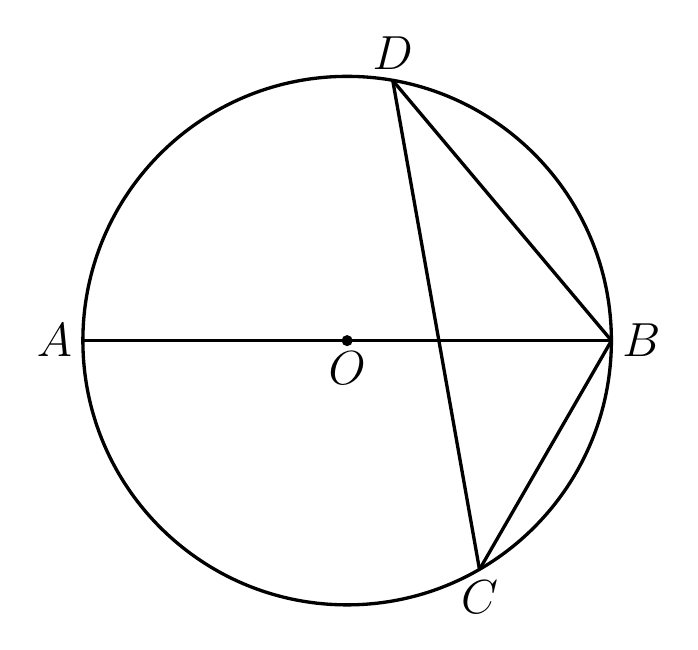
\begin{tikzpicture}[line join=round, line width=1.2pt, font=\fontsize{18}{21.6}\selectfont]
  % Named coordinates (converted from pixels, y flipped)
  \coordinate (O) at (0,0);
  \coordinate (A) at (-3.356,0);
  \coordinate (B) at (3.357,0);
  \coordinate (D) at (0.579,3.304);
  \coordinate (C) at (1.681,-2.907);
  \coordinate (E) at (1.162,0);  % unlabeled intersection

  % Circle centred at O, radius 157.28 px
  \draw (O) circle[radius=3.356];

  % Filled dot at circle centre O (enlarged)
  \fill (O) circle (2pt);

  % Diameter AB
  \draw (A) -- (B);

  % Segments D-B, C-B, D-C (D-C crosses AB at E)
  \draw (D) -- (B);
  \draw (C) -- (B);
  \draw (D) -- (C);

  % Labels (A and B moved level with their endpoints)
  \node[above] at (D) {$D$};
  \node[left] at (A) {$A$};
  \node[right] at (B) {$B$};
  \node[below] at (C) {$C$};
  \node[below] at (O) {$O$};
\end{tikzpicture}
\end{document}